
%{{第五十六回}}{第五十六回}}

\chapter{敏探春兴利除宿弊\\时宝钗小惠全大体}

{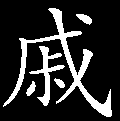
\includegraphics[width=3mm]{../Images/00005}叙入梦景,极迷离,却极分明。牛鬼蛇神不犯笔端,全从至情至理中写出,《齐谐》莫能载也。}

话说平儿陪着凤姐儿吃了饭,伏侍盥漱毕,方往探春处来。只见院中寂静,只有丫鬟婆子诸内壸近人在窗外听候。

平儿进入厅中,他姊妹三人正议论些家务,说的便是年内赖大家请吃酒他家花园中事故。见他来了,探春便命他脚踏上坐了,因说道:``我想的事不为别的,因想着我们一月有二两月银外,丫头们又另有月钱。前儿又有人回,要我们一月所用的头油脂粉,每人又是二两。这又同才刚学里的八两一样,重重叠叠,事虽小,钱有限,看起来也不妥当。你奶奶怎么就没想到这个?''

平儿笑道:``这有个原故:姑娘们所用的这些东西,自然是该有分例。每月买办买了,令女人们各房交与我们收管,不过预备姑娘们使用就罢了,没有一个我们天天各人拿钱找人买头油又是脂粉去的理。所以外头买办总领了去,按月使女人按房交与我们的。姑娘们的每月这二两,原不是为买这些的,原为的是一时当家的奶奶太太或不在,或不得闲,姑娘们偶然一时可巧要几个钱使,省得找人去。这原是恐怕姑娘们受委屈,可知这个钱并不是买这个才有的。如今我冷眼看着,各房里的我们的姊妹都是现拿钱买这些东西的,竟有一半。我就疑惑,不是买办脱了空,迟些日子,就是买的不是正经货,弄些使不得的东西来搪塞。''探春李纨都笑道:``你也留心看出来了。脱空是没有的,也不敢,只是迟些日子;催急了,不知那里弄些来,不过是个名儿,其实使不得,依然得现买。就用这二两银子,另叫别人的奶妈子的或是弟兄哥哥的儿子买了来才使得。若使了官中的人,依然是那一样的。不知他们是什么法子,是铺子里坏了不要的,他们都弄了来,单预备给我们?''平儿笑道:``买办买的是那样的,他买了好的来,买办岂肯和他善开交,又说他使坏心要夺这买办了。所以他们也只得如此,宁可得罪了里头,不肯得罪了外头办事的人。姑娘们只能可使奶妈妈们,他们也就不敢闲话了。''探春道:``因此我心中不自在。钱费两起,东西又白丢一半,通算起来,反费了两折子,不如竟把买办的每月蠲了为是。此是一件事。第二件,年里往赖大家去,你也去的,你看他那小园子比咱们这个如何?''平儿笑道:``还没有咱们这一半大,树木花草也少多了。''探春道:``我因和他家女儿说闲话儿,谁知那么个园子,除他们戴的花、吃的笋菜鱼虾之外,一年还有人包了去,年终足有二百两银子剩。从那日我才知道,一个破荷叶,一根枯草根子,都是值钱的。''

宝钗笑道:``真真膏粱纨绮之谈。虽是千金小姐,原不知这事,但你们都念过书识字的,竟没看见朱夫子有一篇《不自弃文》不成?''探春笑道:``虽看过,那不过是勉人自励,虚比浮词,那里都真有的?''宝钗道:``朱子都有虚比浮词?那句句都是有的。你才办了两天时事,就利欲熏心,把朱子都看虚浮了。你再出去见了那些利弊大事,越发把孔子也看虚了!''探春笑道:``你这样一个通人,竟没看见子书?当日`姬子'有云:`登利禄之场,处运筹之界者,窃尧舜之词,背孔孟之道。'''宝钗笑道:``底下一句呢?''探春笑道:``如今只断章取意,念出底下一句,我自己骂我自己不成?''宝钗道:``天下没有不可用的东西;既可用,便值钱。难为你是个聪敏人,这些正事大节目事竟没经历,也可惜迟了。''{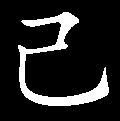
\includegraphics[width=3mm]{../Images/00003}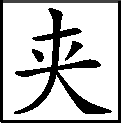
\includegraphics[width=3mm]{../Images/00012}\footnotesize \kaishu 反点题,文法中又一变体也。}李纨笑道:``叫了人家来,不说正事,且你们对讲学问。''宝钗道:``学问中便是正事。此刻于小事上用学问一提,那小事越发作高一层了。不拿学问提着,便都流入市俗去了。''

三人只是取笑之谈,说了笑了一回,便仍谈正事。{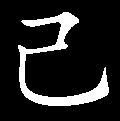
\includegraphics[width=3mm]{../Images/00003}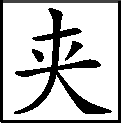
\includegraphics[width=3mm]{../Images/00012}\footnotesize \kaishu 作者又用金蝉脱壳之法。}探春因又接说道:``咱们这园子只算比他们的多一半,加一倍算,一年就有四百银子的利息。若此时也出脱生发银子,自然小器,不是咱们这样人家的事。若派出两个一定的人来,既有许多值钱之物,一味任人作践,也似乎暴殄天物。不如在园子里所有的老妈妈中,拣出几个本分老诚能知园圃的事,派准他们收拾料理,也不必要他们交租纳税,只问他们一年可以孝敬些什么。一则园子有专定之人修理,花木自有一年好似一年的,也不用临时忙乱;二则也不至作践,白辜负了东西;三则老妈妈们也可借此小补,不枉年日在园中辛苦;四则亦可以省了这些花儿匠山子匠打扫人等的工费。将此有馀,以补不足,未为不可。''宝钗正在地下看壁上的字画,听如此说一则,便点一回头,说完,便笑道:``善哉,三年之内无饥馑矣!''李纨笑道:``好主意。这果一行,太太必喜欢。省钱事小,第一有人打扫,专司其职,又许他们去卖钱。使之以权,动之以利,再无不尽职的了。''平儿道:``这件事须得姑娘说出来。我们奶奶虽有此心,也未必好出口。此刻姑娘们在园里住着,不能多弄些玩意儿去陪衬,反叫人去监管修理,图省钱,这话断不好出口。''

宝钗忙走过来,摸着他的脸笑道:``你张开嘴,我瞧瞧你的牙齿舌头是什么作的。从早起来到这会子,你说这些话,一套一个样子,也不奉承三姑娘,也没见你说奶奶才短想不到,也并没有三姑娘说一句,你就说一句是;横竖三姑娘一套话出,你就有一套话进去;总是三姑娘想的到的,你奶奶也想到了,只是必有个不可办的原故。这会子又是因姑娘住的园子,不好因省钱令人去监管。你们想想这话,若果真交与人弄钱去的,那人自然是一枝花也不许掐,一个果子也不许动了,姑娘们分中自然不敢,天天与小姑娘们就吵不清。他这远愁近虑,不亢不卑。他奶奶便不是和咱们好,听他这一番话,也必要自愧的变好了,不和也变和了。''探春笑道:``我早起一肚子气,听他来了,忽然想起他主子来,素日当家使出来的好撒野的人,我见了他便生了气。谁知他来了,避猫鼠儿似的站了半日,怪可怜的。接着又说了那么些话,不说他主子待我好,倒说`不枉姑娘待我们奶奶素日的情意了'。这一句,不但没了气,我倒愧了,又伤起心来。我细想,我一个女孩儿家,自己还闹得没人疼没人顾的,我那里还有好处去待人。''口内说到这里,不免又流下泪来。李纨等见他说的恳切,又想他素日赵姨娘每生诽谤,在王夫人跟前亦为赵姨娘所累,亦都不免流下泪来,都忙劝道:``趁今日清净,大家商议两件兴利剔弊的事,也不枉太太委托一场。又提这没要紧的事做什么?''平儿忙道:``我已明白了。姑娘竟说谁好,竟一派人就完了。''探春道:``虽如此说,也须得回你奶奶一声。我们这里搜剔小遗,已经不当,皆因你奶奶是个明白人,我才这样行,若是糊涂多蛊多妒的,我也不肯,倒像抓他乖一般。岂可不商议了行。''平儿笑道:``既这样,我去告诉一声。''说着去了,半日方回来,笑说:``我说是白走一趟,这样好事,奶奶岂有不依的。''

探春听了,便和李纨命人将园中所有婆子的名单要来,大家参度,大概定了几个。又将他们一齐传来,李纨大概告诉与他们。众人听了,无不愿意,也有说:``那一片竹子单交给我,一年工夫,明年又是一片。除了家里吃的笋,一年还可交些钱粮。''这一个说:``那一片稻地交给我,一年这些顽的大小雀鸟的粮食不必动官中钱粮,我还可以交钱粮。''探春才要说话,人回:``大夫来了,进园瞧姑娘。''众婆子只得去接大夫。平儿忙说:``单你们,有一百个也不成个体统,难道没有两个管事的头脑带进大夫来?''回事的那人说:``有,吴大娘和单大娘他两个在西南角上聚锦门等着呢。''平儿听说,方罢了。

众婆子去后,探春问宝钗如何。宝钗笑答道:``幸于始者怠于终,缮其辞者嗜其利。''探春听了点头称赞,便向册上指出几人来与他三人看。平儿忙去取笔砚来。他三人说道:``这一个老祝妈是个妥当的,况他老头子和他儿子代代都是管打扫竹子,如今竟把这所有的竹子交与他。这一个老田妈本是种庄稼的,稻香村一带凡有菜蔬稻稗之类,虽是顽意儿,不必认真大治大耕,也须得他去,再一按时加些培植,岂不更好?''探春又笑道:``可惜,蘅芜苑和怡红院这两处大地方竟没有出利息之物。''李纨忙笑道:``蘅芜苑更利害。如今香料铺并大市大庙卖的各处香料香草儿,都不是这些东西?算起来比别的利息更大。怡红院别说别的,单只说春夏天一季玫瑰花,共下多少花?还有一带篱笆上蔷薇、月季、宝相、金银藤,单这没要紧的草花干了,卖到茶叶铺药铺去,也值几个钱。''探春笑道:``原来如此。只是弄香草的没有在行的人。''平儿忙笑道:``跟宝姑娘的莺儿他妈就是会弄这个的,上回他还采了些晒干了编成花篮葫芦给我顽的,姑娘倒忘了不成?''宝钗笑道:``我才赞你,你倒来捉弄我了。''三人都诧异,都问这是为何。宝钗道:``断断使不得!你们这里多少得用的人,一个一个闲着没事办,这会子我又弄个人来,叫那起人连我也看小了。我倒替你们想出一个人来:怡红院有个老叶妈,他就是茗烟的娘。那是个诚实老人家,他又和我们莺儿的娘极好,不如把这事交与叶妈。他有不知的,不必咱们说,他就找莺儿的娘去商议了。那怕叶妈全不管,竟交与那一个,那是他们私情儿,有人说闲话,也就怨不到咱们身上了。如此一行,你们办的又至公,于事又甚妥。''李纨平儿都道:``是极。''{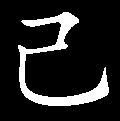
\includegraphics[width=3mm]{../Images/00003}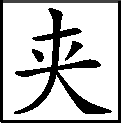
\includegraphics[width=3mm]{../Images/00012}\footnotesize \kaishu 宝钗此等非与凤姐一样,此是随时俯仰,彼则逸才逾蹈也。}探春笑道:``虽如此,只怕他们见利忘义。''{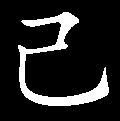
\includegraphics[width=3mm]{../Images/00003}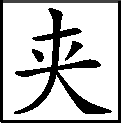
\includegraphics[width=3mm]{../Images/00012}\footnotesize \kaishu 这是探春敏智过人处,此讽亦不可少。}平儿笑道:``不相干,前儿莺儿还认了叶妈做干娘,请吃饭吃酒,两家和厚的好的很呢。''{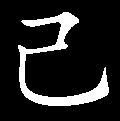
\includegraphics[width=3mm]{../Images/00003}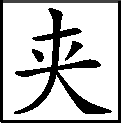
\includegraphics[width=3mm]{../Images/00012}\footnotesize \kaishu 夹写大观园中多少儿女家常闲景,此亦补前文之不足也。}探春听了,方罢了。又共同斟酌出几人来,俱是他四人素昔冷眼取中的,用笔圈出。

一时婆子们来回大夫已去,将药方送上去。三人看了,一面遣人送出去取药,监派调服,一面探春与李纨明示诸人:某人管某处,按四季除家中定例用多少外,馀者任凭你们采取了去取利,年终算账。探春笑道:``我又想起一件事:若年终算账归钱时,自然归到账房,仍是上头又添一层管主,还在他们手心里,又剥一层皮。这如今我们兴出这事来派了你们,已是跨过他们的头去了,心里有气,只说不出来;你们年终去归账,他还不捉弄你们等什么?再者,这一年间管什么的,主子有一全分,他们就得半分。这是家里的旧例,人所共知的,别的偷着的在外。如今这园子里是我的新创,竟别入他们手,每年归账,竟归到里头来才好。''宝钗笑道:``依我说,里头也不用归账。这个多了那个少了,倒多了事。不如问他们谁领这一分的,他就揽一宗事去。不过是园里的人的动用。我替你们算出来了,有限的几宗事:不过是头油、胭粉、香、纸,每一位姑娘几个丫头,都是有定例的;再者,各处笤帚、撮簸、掸子并大小禽鸟、鹿、兔吃的粮食。不过这几样,都是他们包了去,不用账房去领钱。你算算,就省下多少来?''平儿笑道:``这几宗虽小,一年通共算了,也省的下四百两银子。''

宝钗笑道:``却又来,一年四百,二年八百两,取租的房子也能看得了几间,薄地也可添几亩。虽然还有敷馀的,但他们既辛苦闹一年,也要叫他们剩些,粘补粘补自家。虽是兴利节用为纲,然亦不可太啬。纵再省上二三百银子,失了大体统也不像。所以如此一行,外头账房里一年少出四五百银子,也不觉得很艰啬了,他们里头却也得些小补。这些没营生的妈妈们也宽裕了,园子里花木,也可以每年滋长蕃盛,你们也得了可使之物。这庶几不失大体。若一味要省时,那里不搜寻出几个钱来。凡有些馀利的,一概入了官中,那时里外怨声载道,岂不失了你们这样人家的大体?如今这园里几十个老妈妈们,若只给了这个,那剩的也必抱怨不公。我才说的,他们只供给这个几样,也未免太宽裕了。一年竟除这个之外,他每人不论有馀无馀,只叫他拿出若干贯钱来,大家凑齐,单散与园中这些妈妈们。他们虽不料理这些,却日夜也是在园中照看当差之人,关门闭户,起早睡晚,大雨大雪,姑娘们出入,抬轿子,撑船,拉冰床,一应粗糙活计,都是他们的差使。一年在园里辛苦到头,这园内既有出息,也是分内该沾带些的。还有一句至小的话,越发说破了:你们只管了自己宽裕,不分与他们些,他们虽不敢明怨,心里却都不服,只用假公济私的多摘你们几个果子,多掐几枝花儿,你们有冤还没处诉。他们也沾带了些利息,你们有照顾不到,他们就替你照顾了。''

众婆子听了这个议论,又去了账房受辖制,又不与凤姐儿去算账,一年不过多拿出若干贯钱来,各各欢喜异常,都齐说:``愿意。强如出去被他揉搓着,还得拿出钱来呢。''那不得管地的听了每年终又无故得分钱,也都喜欢起来,口内说:``他们辛苦收拾,是该剩些钱粘补的。我们怎么好`稳坐吃三注'的?''

宝钗笑道:``妈妈们也别推辞了,这原是分内应当的。你们只要日夜辛苦些,别躲懒纵放人吃酒赌钱就是了。不然,我也不该管这事;你们一般听见,姨娘亲口嘱托我三五回,说大奶奶如今又不得闲儿,别的姑娘又小,托我照看照看。我若不依,分明是叫姨娘操心。你们奶奶又多病多痛,家务也忙。我原是个闲人,便是个街坊邻居,也要帮着些,何况是亲姨娘托我。我免不得去小就大,讲不起众人嫌我。倘或我只顾了小分沽名钓誉,那时酒醉赌博生出事来,我怎么见姨娘?你们那时后悔也迟了,就连你们素日的老脸也都丢了。这些姑娘小姐们,这么一所大花园子,都是你们照看,皆因看得你们是三四代的老妈妈,最是循规遵矩的,原该大家齐心,顾些体统。你们反纵放别人任意吃酒赌博,姨娘听见了,教训一场犹可,倘或被那几个管家娘子听见了,他们也不用回姨娘,竟教导你们一番。你们这年老的反受了年小的教训,虽是他们是管家,管的着你们,何如自己存些体统,他们如何得来作践。所以我如今替你们想出这个额外的进益来,也为大家齐心把这园里周全的谨谨慎慎,使那些有权执事的看见这般严肃谨慎,且不用他们操心,他们心里岂不敬伏。也不枉替你们筹画进益,既能夺他们之权,生你们之利,岂不能行无为之治,分他们之忧。你们去细想想这话。''家人都欢声鼎沸说:``姑娘说的很是。从此姑娘奶奶只管放心,姑娘奶奶这样疼顾我们,我们再要不体上情,天地也不容了。''

刚说着,只见林之孝家的进来说:``江南甄府里家眷昨日到京,今日进宫朝贺。此刻先遣人来送礼请安。''说着,便将礼单送上去。探春接了,看道是:``上用的妆缎蟒缎十二匹,上用杂色缎十二匹,上用各色纱十二匹,上用宫绸十二匹,官用各色缎纱绸绫二十四匹。''\href{../Text/part0060_split_000.html\#lnkback_1_a}{\textsuperscript{①}}李纨也看过,说:``用上等封儿赏他。''因又命人回了贾母。贾母便命人叫李纨、探春、宝钗等也都过来,将礼物看了。李纨收过,一边吩咐内库上人说:``等太太回来看了再收。''贾母因说:``这甄家又不与别家相同,上等赏封赏男人,只怕展眼又打发女人来请安,预备下尺头。''一语未完,果然人回:``甄府四个女人来请安。''贾母听了,忙命人带进来。

那四个人都是四十往上的年纪,穿戴之物,皆比主子不甚差别。请安问好毕,贾母命拿了四个脚踏来,他四人谢了坐,待宝钗等坐了,方都坐下。贾母便问:``多早晚进京的?''四人忙起身回说:``昨儿进的京。今日太太带了姑娘进宫请安去了,故令女人们来请安,问候姑娘们。''贾母笑问道:``这些年没进京,也不想到今年来。''四人也都笑回道:``正是,今年是奉旨进京的。''贾母问道:``家眷都来了?''四人回说:``老太太和哥儿、两位小姐并别位太太都没来,就只太太带了三姑娘来了。''贾母道:``有人家没有?''四人道:``尚没有。''贾母笑道:``你们大姑娘和二姑娘这两家,都和我们家甚好。''四人笑道:``正是。每年姑娘们有信回去说,全亏府上照看。''贾母笑道:``什么照看,原是世交,又是老亲,原应当的。你们二姑娘更好,更不自尊自大,所以我们才走的亲密。''四人笑道:``这是老太太过谦了。''贾母又问:``你这哥儿也跟着你们老太太?''四人回说:``也是跟着老太太。''贾母道:``几岁了?''又问:``上学不曾?''四人笑说:``今年十三岁。因长得齐整,老太太很疼。自幼淘气异常,天天逃学,老爷太太也不便十分管教。''贾母笑道:``也不成了我们家的了!你这哥儿叫什么名字?''四人道:``因老太太当作宝贝一样,他又生的白,老太太便叫作宝玉。''贾母便向李纨等道:``偏也叫作个宝玉。''李纨忙欠身笑道:``从古至今,同时隔代重名的很多。''四人也笑道:``起了这小名儿之后,我们上下都疑惑,不知那位亲友家也倒似曾有一个的。只是这十来年没进京来,却记不得真了。''贾母笑道:``岂敢,就是我的孙子。------人来。''众媳妇丫头答应了一声,走近几步。贾母笑道:``园里把咱们的宝玉叫了来,给这四个管家娘子瞧瞧,比他们的宝玉如何?''

众媳妇听了,忙去了,半刻围了宝玉进来。四人一见,忙起身笑道:``唬了我们一跳。若是我们不进府来,倘若别处遇见,还只道我们的宝玉后赶着也进了京了呢。''一面说,一面都上来拉他的手,问长问短。宝玉忙也笑问好。贾母笑道:``比你们的长的如何?''李纨等笑道:``四位妈妈才一说,可知是模样相仿了。''贾母笑道:``那有这样巧事?大家子孩子们再养的娇嫩,除了脸上有残疾十分黑丑的,大概看去都是一样的齐整。这也没有什么怪处。''四人笑道:``如今看来,模样是一样。据老太太说,淘气也一样。我们看来,这位哥儿性情却比我们的好些。''贾母忙问:``怎见得?''四人笑道:``方才我们拉哥儿的手说话便知。我们那一个只说我们糊涂,慢说拉手,他的东西我们略动一动也不依。所使唤的人都是女孩子们。''四人未说完,李纨姊妹等禁不住都失声笑出来。贾母也笑道:``我们这会子也打发人去见了你们宝玉,若拉他的手,他也自然勉强忍耐一时。可知你我这样人家的孩子们,凭他们有什么刁钻古怪的毛病儿,见了外人,必是要还出正经礼数来的。若他不还正经礼数,也断不容他刁钻去了。就是大人溺爱的,是他一则生的得人意,二则见人礼数竟比大人行出来的不错,使人见了可爱可怜,背地里所以才纵他一点子。若一味他只管没里没外,不与大人争光,凭他生的怎样,也是该打死的。''四人听了,都笑道:``老太太这话正是。虽然我们宝玉淘气古怪,有时见了人客,规矩礼数更比大人有礼。所以无人见了不爱,只说为什么还打他。殊不知他在家里无法无天,大人想不到的话偏会说,想不到的事他偏要行,所以老爷太太恨的无法。就是弄性,也是小孩子的常情,胡乱花费,这也是公子哥儿的常情,怕上学,也是小孩子的常情,都还治的过来。第一,天生下来这一种刁钻古怪的脾气,如何使得。''一语未了,人回:``太太回来了。''王夫人进来问过安。他四人请了安,大概说了两句。贾母便命歇歇去。王夫人亲捧过茶,方退出。四人告辞了贾母,便往王夫人处来,说了一会家务,打发他们回去,不必细说。

这里贾母喜的逢人便告诉,也有一个宝玉,也却一般行景。众人都为天下之大,世宦之多,同名者也甚多,祖母溺爱孙者也古今所有常事耳,不是什么罕事,故皆不介意。独宝玉是个迂阔呆公子的性情,自为是那四人承悦贾母之词。后至蘅芜苑去看湘云病去,史湘云说他:``你放心闹罢,先是`单丝不成线,独树不成林',如今有了个对子,闹急了,再打很了,你逃走到南京找那一个去。''宝玉道:``那里的谎话你也信了,偏又有个宝玉了?''湘云道:``怎么列国有个蔺相如,汉朝又有个司马相如呢?''宝玉笑道:``这也罢了,偏又模样儿也一样,这是没有的事。''湘云道:``怎么匡人看见孔子,只当是阳虎呢?''宝玉笑道:``孔子、阳虎虽同貌,却不同名;蔺与司马虽同名,而又不同貌;偏我和他就两样俱同不成?''湘云没了话答对,因笑道:``你只会胡搅,我也不和你分证。有也罢,没也罢,与我无干。''说着便睡下了。

宝玉心中便又疑惑起来:若说必无,然亦似有;若说必有,又并无目睹。心中闷了,回至房中榻上默默盘算,不觉就忽忽的睡去,不觉竟到了一座花园之内。宝玉诧异道:``除了我们大观园,竟又有这一个园子?''{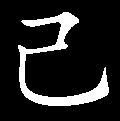
\includegraphics[width=3mm]{../Images/00003}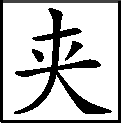
\includegraphics[width=3mm]{../Images/00012}\footnotesize \kaishu 写园可知。}正疑惑间,从那边来了几个女儿,都是丫鬟。宝玉又诧异道:``除了鸳鸯、袭人、平儿之外,也竟还有这一干人?''{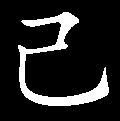
\includegraphics[width=3mm]{../Images/00003}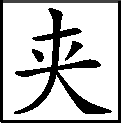
\includegraphics[width=3mm]{../Images/00012}\footnotesize \kaishu 写人可知。妙在并不说``更强''二字。}只见那些丫鬟笑道:``宝玉怎么跑到这里来了?''宝玉只当是说他,自己忙来陪笑说道:``因我偶步到此,不知是那位世交的花园,好姐姐们,带我逛逛。''众丫鬟都笑道:``原来不是咱家的宝玉。他生的倒也还干净,{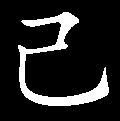
\includegraphics[width=3mm]{../Images/00003}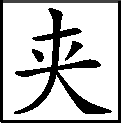
\includegraphics[width=3mm]{../Images/00012}\footnotesize \kaishu 妙。在玉卿身上只落了这两个字,亦不奇了。}嘴儿也倒乖觉。''宝玉听了,忙道:``姐姐们,这里也更还有个宝玉?''丫鬟们忙道:``宝玉二字,我们是奉老太太、太太之命,为保佑他延寿消灾的。我叫他,他听见喜欢。你是那里远方来的臭小厮,也乱叫起他来。仔细你的臭肉,打不烂你的。''又一个丫鬟笑道:``咱们快走罢,别叫宝玉看见,又说同这臭小厮说了话,把咱熏臭了。''说着一径去了。

宝玉纳闷道:``从来没有人如此涂毒我,他们如何更这样?真亦有我这样一个人不成?''一面想,一面顺步早到了一所院内。宝玉又诧异道:``除了怡红院,也更还有这么一个院落。''忽上了台矶,进入屋内,只见榻上有一个人卧着,那边有几个女孩儿做针线,也有嘻笑顽耍的。只见榻上那个少年叹了一声。一个丫鬟笑问道:``宝玉,你不睡又叹什么?想必为你妹妹病了,你又胡愁乱恨呢。''宝玉听说,心下也便吃惊。只见榻上少年说道:``我听见老太太说,长安都中也有个宝玉,和我一样的性情,我只不信。我才作了一个梦,竟梦中到了都中一个花园子里头,遇见几个姐姐,都叫我臭小厮,不理我。好容易找到他房里头,偏他睡觉,空有皮囊,真性不知那去了。''宝玉听说,忙说道:``我因找宝玉来到这里。原来你就是宝玉?''榻上的忙下来拉住:``原来你就是宝玉?这可不是梦里了。''宝玉道:``这如何是梦?真且又真了。''一语未了,只见人来说:``老爷叫宝玉。''唬得二人皆慌了。一个宝玉就走,一个宝玉便忙叫:``宝玉快回来,快回来!''

袭人在旁听他梦中自唤,忙推醒他,笑问道:``宝玉在那里?''此时宝玉虽醒,神意尚恍惚,因向门外指说:``才出去了。''袭人笑道:``那是你梦迷了。你揉眼细瞧,是镜子里照的你影儿。''宝玉向前瞧了一瞧,原是那嵌的大镜对面相照,自己也笑了。早有人捧过漱盂茶卤来,漱了口。麝月道:``怪道老太太常嘱咐说小人屋里不可多有镜子。小人魂不全,有镜子照多了,睡觉惊恐作胡梦。如今倒在大镜子那里安了一张床。有时放下镜套还好;往前去,天热困倦不定,那里想的到放他,比如方才就忘了。自然是先躺下照着影儿顽的,一时合上眼,自然是胡梦颠倒;不然如何得看着自己叫着自己的名字?不如明儿挪进床来是正经。''一语未了,只见王夫人遣人来叫宝玉,不知有何话说------{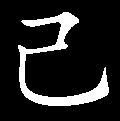
\includegraphics[width=3mm]{../Images/00003}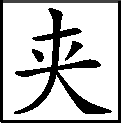
\includegraphics[width=3mm]{../Images/00012}\footnotesize \kaishu 此下紧接``慧紫鹃试忙玉''。}

{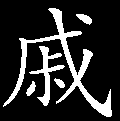
\includegraphics[width=3mm]{../Images/00005}总评:探春看得透,拿得定,说得出,办得来,是有才干者,故赠以``敏''字;宝钗认的真,用的当,责的专,待的厚,是善知人者,故赠以``识''字。}\href{../Text/part0060_split_000.html\#lnkback_2_a}{\textsuperscript{②}}{``敏''与``识''合,何事不济?}

{叙园圃事极板重,却极活泼。营心孔方,带以图记,劳形案牍,不费讴吟。高人焉肯以书香混于铜臭也哉!}

% {\href{../Text/part0060_split_000.html\#navto_1_a}{①}此礼单戚、蒙、杨本与诸本不同,作:``上等的妆缎蟒缎十二匹,上用各色宁绸十二匹,上用宫绸十二匹,上用缎十二匹,上用纱十二匹,上用各色绸绫四十匹。''}

% {\href{../Text/part0060_split_000.html\#navto_2_a}{②}按:本回回目``时宝钗'',戚、蒙本作``识宝钗''。}
